\documentclass[a4paper,10pt]{article}

\usepackage[UTF8]{ctex}
\usepackage{tikz}
\usepackage{color}
\usepackage{graphicx}
\usepackage{amsmath}
\usepackage{amssymb}
\usepackage{ulem}
\renewcommand{\baselinestretch}{1.4}
\setcounter{tocdepth}{1}

\begin{document}

\title{ix35 题目集}
\author{ix35}
\date{June 2023}
\maketitle

\pagenumbering{roman}
\tableofcontents
\newpage
\pagenumbering{arabic}

\vspace*{\fill}

{\centering\section*{说明}}

能公开的题目基本都公开了,但有一些题目不适合公开(如 xmoj,洛谷省选计划,ZROI 的题目),这里将不会提供它们的题面和题解。为了避免一些不必要的麻烦,有些题目的用途没有写全,主要是联测题若被用到其他地方则不会再标注联测。

由于题目描述和数据范围是直接从题面里截出来的,所以有的数据范围里的变量在题目描述里找不到,但是多半可以脑补出来。

题面并非全部是从公开版题面中取的,因此可能有些大家没见过的题面。

题目大致以时间排序,但也有一定的随意性。

红色的是觉得出得很好的题。

最好不要问我:为什么我做到的你出的某某题不在这里啊?

大量图片来源于网络,侵删。

\vspace*{\fill}

\newpage

\vspace*{\fill}
\begin{center}

\section{脑力}

\subsection*{2020.1}

\vspace{10pt}

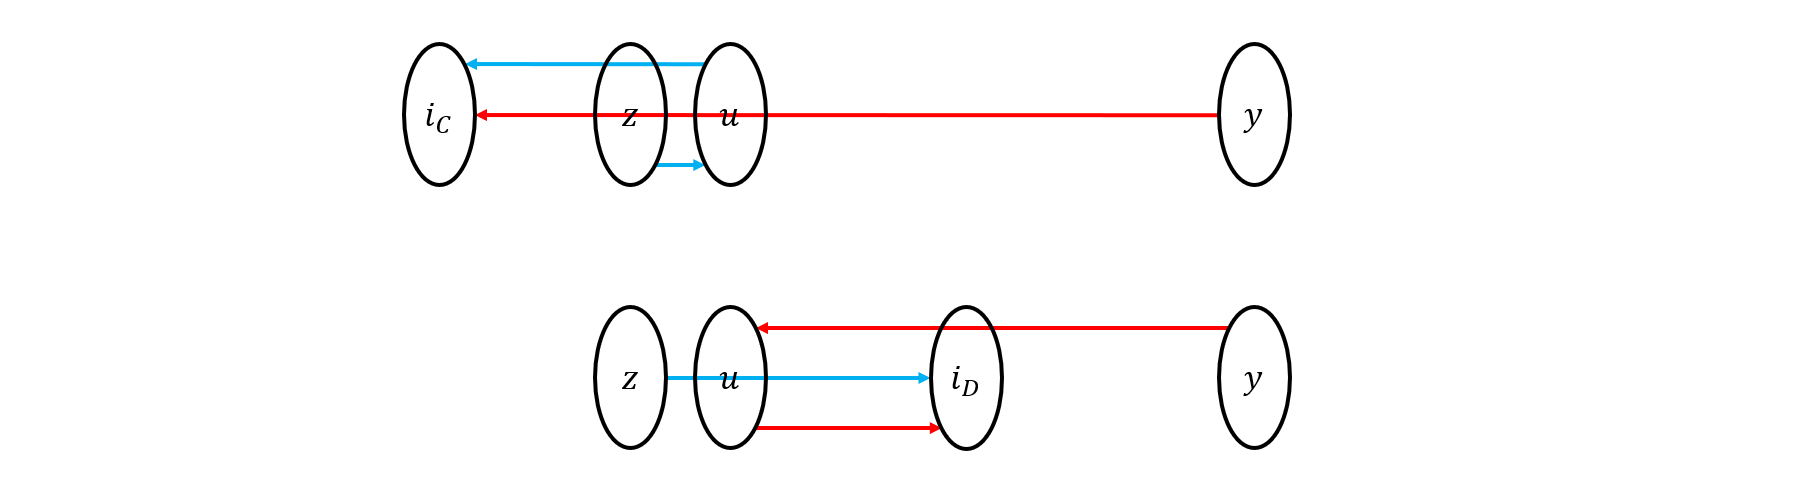
\includegraphics[height=6cm]{../source/pic2.png}

\vspace{10pt}

\textbf{其他名称}:无

\vspace{10pt}

\textbf{用途}:联测

\vspace{10pt}

\textbf{提交方式}:无

\vspace{10pt}

\textbf{难度}:$4/10$

\vspace{10pt}

\textbf{Tag}:字符串,计数

\end{center}
\vspace*{\fill}

\newpage

\section*{背景}

本题是一道很早就出了的题,原本将放到 MdOI R1 中作为 C 题,然而偶然与九条可怜所出的一道模拟赛题撞题,因此改投联测。

题目名称来自音游曲 Brainpower,希望大家都听过 Brainpower 了。

\section*{题目描述}

我们定义:

1. 一句歌词是一个长度为 $m$ 的,仅由小写字母构成的字符串;

2. 一首歌曲是一个由 $n$ 句歌词组成的字符串序列;

3. 一首歌曲的 $\text{san}$ 值为:将所有歌词插入一棵字典树上,该字典树的结点数量。

显然,一首歌曲的各句歌词重复率越高,就越容易洗脑,也就是说 $\text{san}$ 值越低越容易洗脑。

现在给定一首歌曲,由于被洗脑后 ix35 的 $\text{san}$ 值很低,所以他忘记了歌词中的某些位置,现在他想要知道:如果这些被忘记的位置随机选择一个小写字母填上,整首歌曲 $\text{san}$ 值的期望是多少?

答案对 $998244353$ 取模。

\section*{数据范围}

$1\leq n\leq 12,\ 1 \leq m\leq 1000$

\newpage

\vspace*{\fill}
\begin{center}

\section{Treequery}

\subsection*{2020.1}

\vspace{10pt}

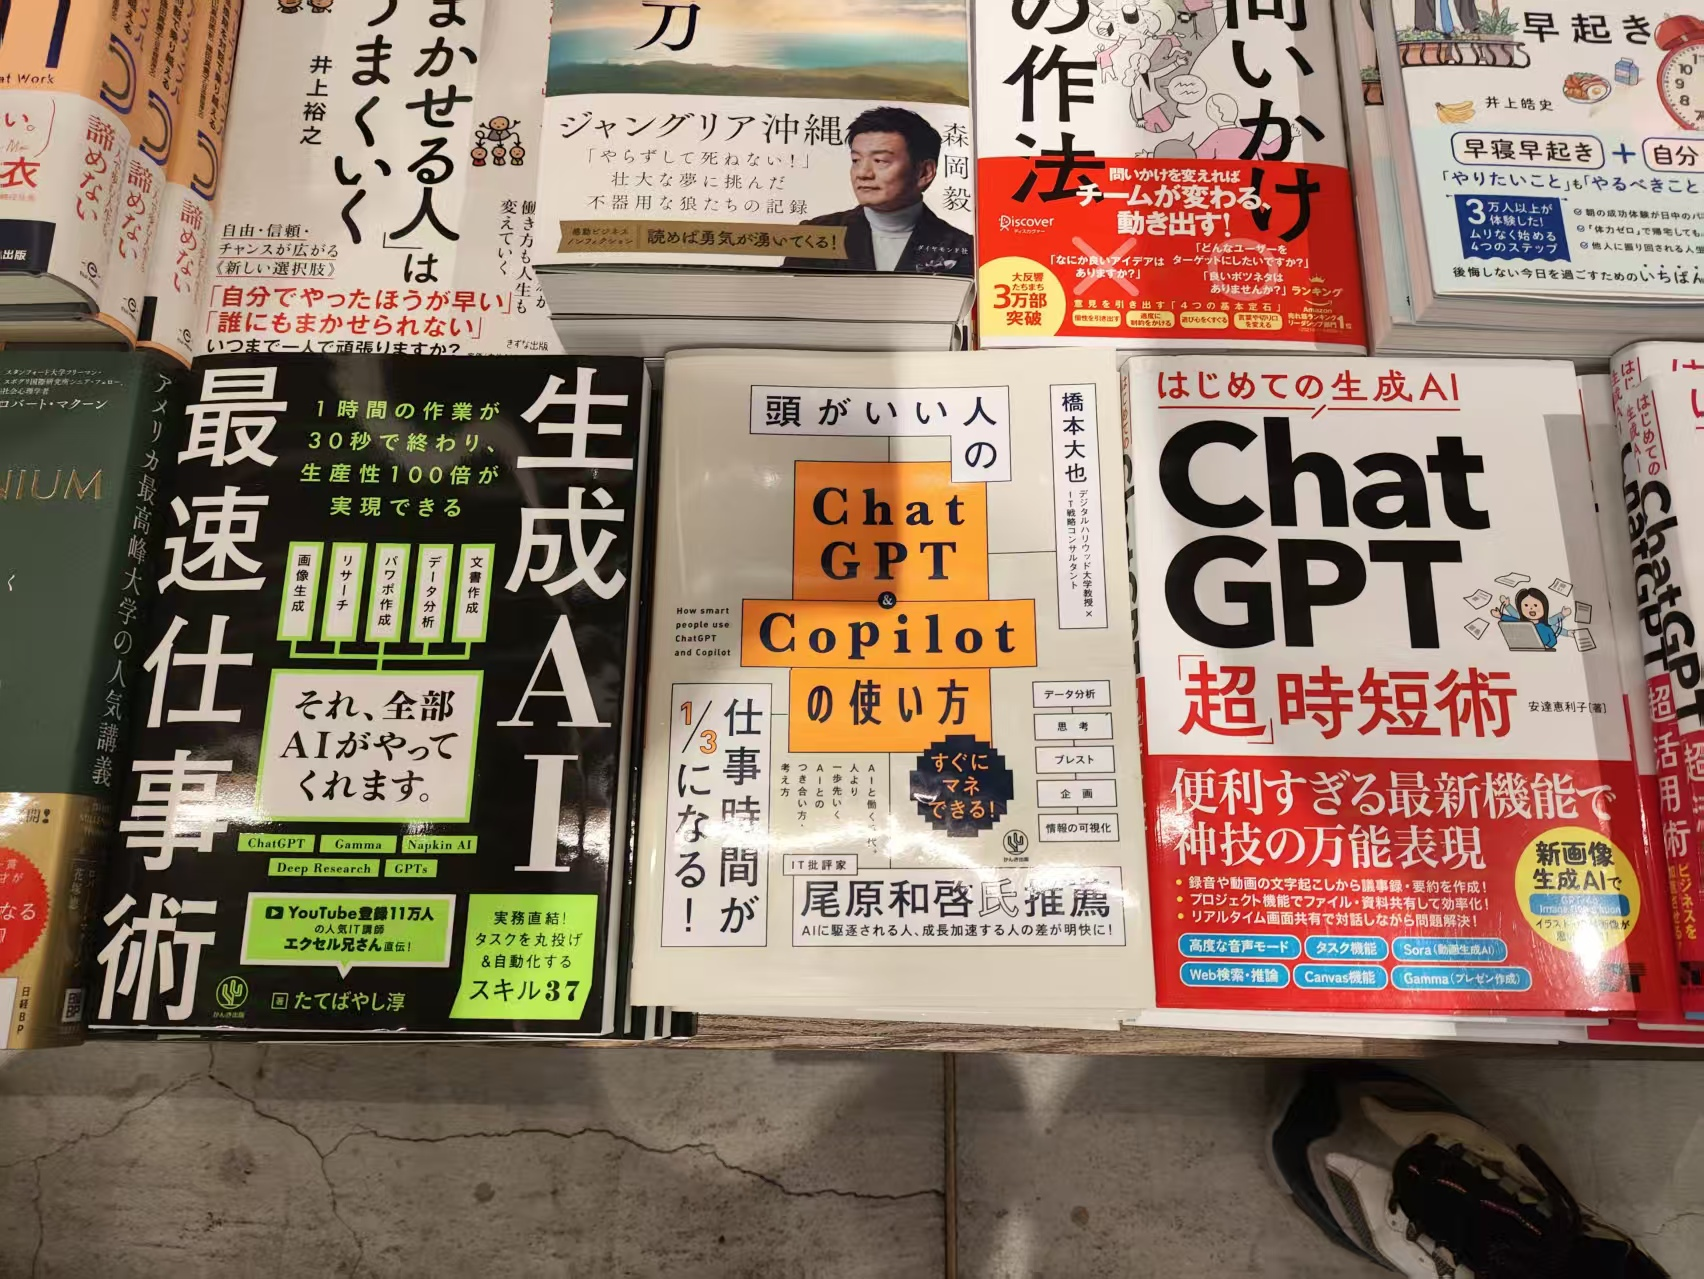
\includegraphics[height=6cm]{../source/pic3.png}

\vspace{10pt}

\textbf{其他名称}:孤程

\vspace{10pt}

\textbf{用途}:MdOI R1 D

\vspace{10pt}

\textbf{提交方式}:Luogu P6071

\vspace{10pt}

\textbf{难度}:$6/10$

\vspace{10pt}

\textbf{Tag}:数据结构

\end{center}
\vspace*{\fill}

\newpage

\section*{背景}

这也是一道很早前就出的题,由于 MdOI R1 差一道题所以就当作了其 D 题。题面由 xht37 润色。

\section*{题目描述}

给定一棵 $n$ 个点的无根树,边有边权。

令 $E(x,y)$ 表示树上 $x,y$ 之间的简单路径上的所有边的集合,特别地,当 $x=y$ 时,$E(x,y)=\varnothing$。

你需要\textbf{实时}回答 $q$ 个询问,每个询问给定 $p,l,r$,请你求出集合 $\bigcap_{i=l}^r E(p,i)$ 中所有边的边权和,即 $E(p, l\dots r)$ 的交所包含的边的边权和。

通俗的讲,你需要求出 $p$ 到 $[l,r]$ 内每一个点的简单路径的公共部分长度。

\section*{数据范围}

$1\leq n,q\leq 2\times 10^5,\ 1\leq x,y,p\leq n,\ 1\leq l\leq r\leq n,\ 1\leq w\leq 10^4$

\newpage

\vspace*{\fill}
\begin{center}

\section{Path}

\subsection*{2020.1}

\vspace{10pt}

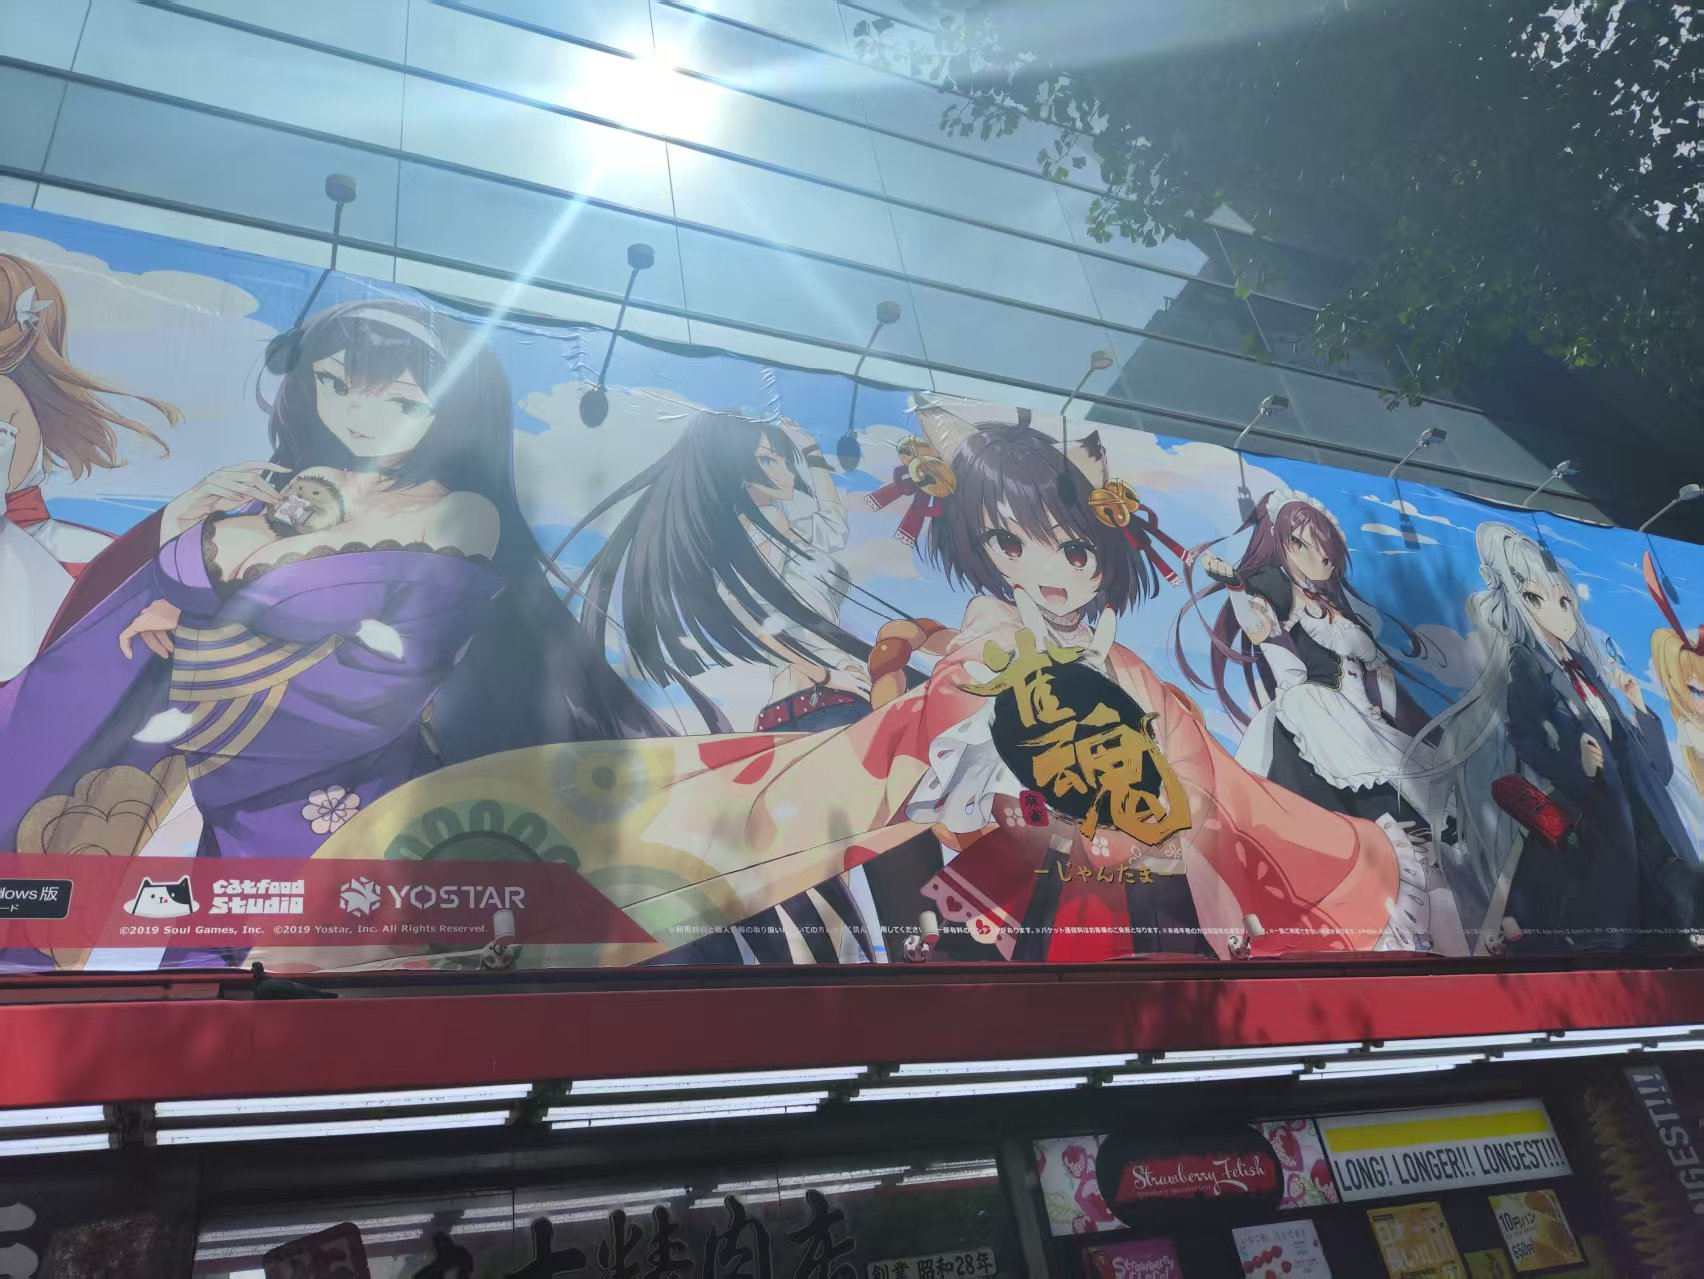
\includegraphics[height=6cm]{../source/pic4.png}

\vspace{10pt}

\textbf{其他名称}:无

\vspace{10pt}

\textbf{用途}:MdOI R1 E

\vspace{10pt}

\textbf{提交方式}:Luogu P6072

\vspace{10pt}

\textbf{难度}:$6/10$

\vspace{10pt}

\textbf{Tag}:数据结构

\end{center}
\vspace*{\fill}

\newpage

\section*{背景}

本题原解法是回滚莫队,但被 lxl 指出存在 $\operatorname{polylog}$ 做法,可见洛谷题解。

题面由 xht37 润色。

\section*{题目描述}

给定一棵 $n$ 个点的无根树,边有边权。

令 $V(x,y),E(x,y)$ 分别表示树上 $x,y$ 之间的简单路径上的所有点的集合和所有边的集合,特别地,当 $x=y$ 时,$V(x,y) = \{x\}$,$E(x,y)=\varnothing$。

再令边集 $E$ 的权值 $f(E)$ 为 $E$ 中所有边的权值的\textbf{异或和},当 $E=\varnothing$ 时,$f(E) = 0$。

现在,要你求出:

$$
\max_{1\le x,y,u,v \le n,V(x,y)\cap V(u,v)=\varnothing}(f(E(x,y)) + f(E(u,v)))
$$

通俗的讲,你要选择两条简单路径,满足没有重合的点,且边权异或和之和最大。

\section*{数据范围}

$2\leq n\leq 3\times 10^4,\ 1\leq x,y\leq n,\ 0\leq w\leq 10^9$

\newpage

\vspace*{\fill}
\begin{center}

\section{Odyssey}

\subsection*{2020.4}

\vspace{10pt}

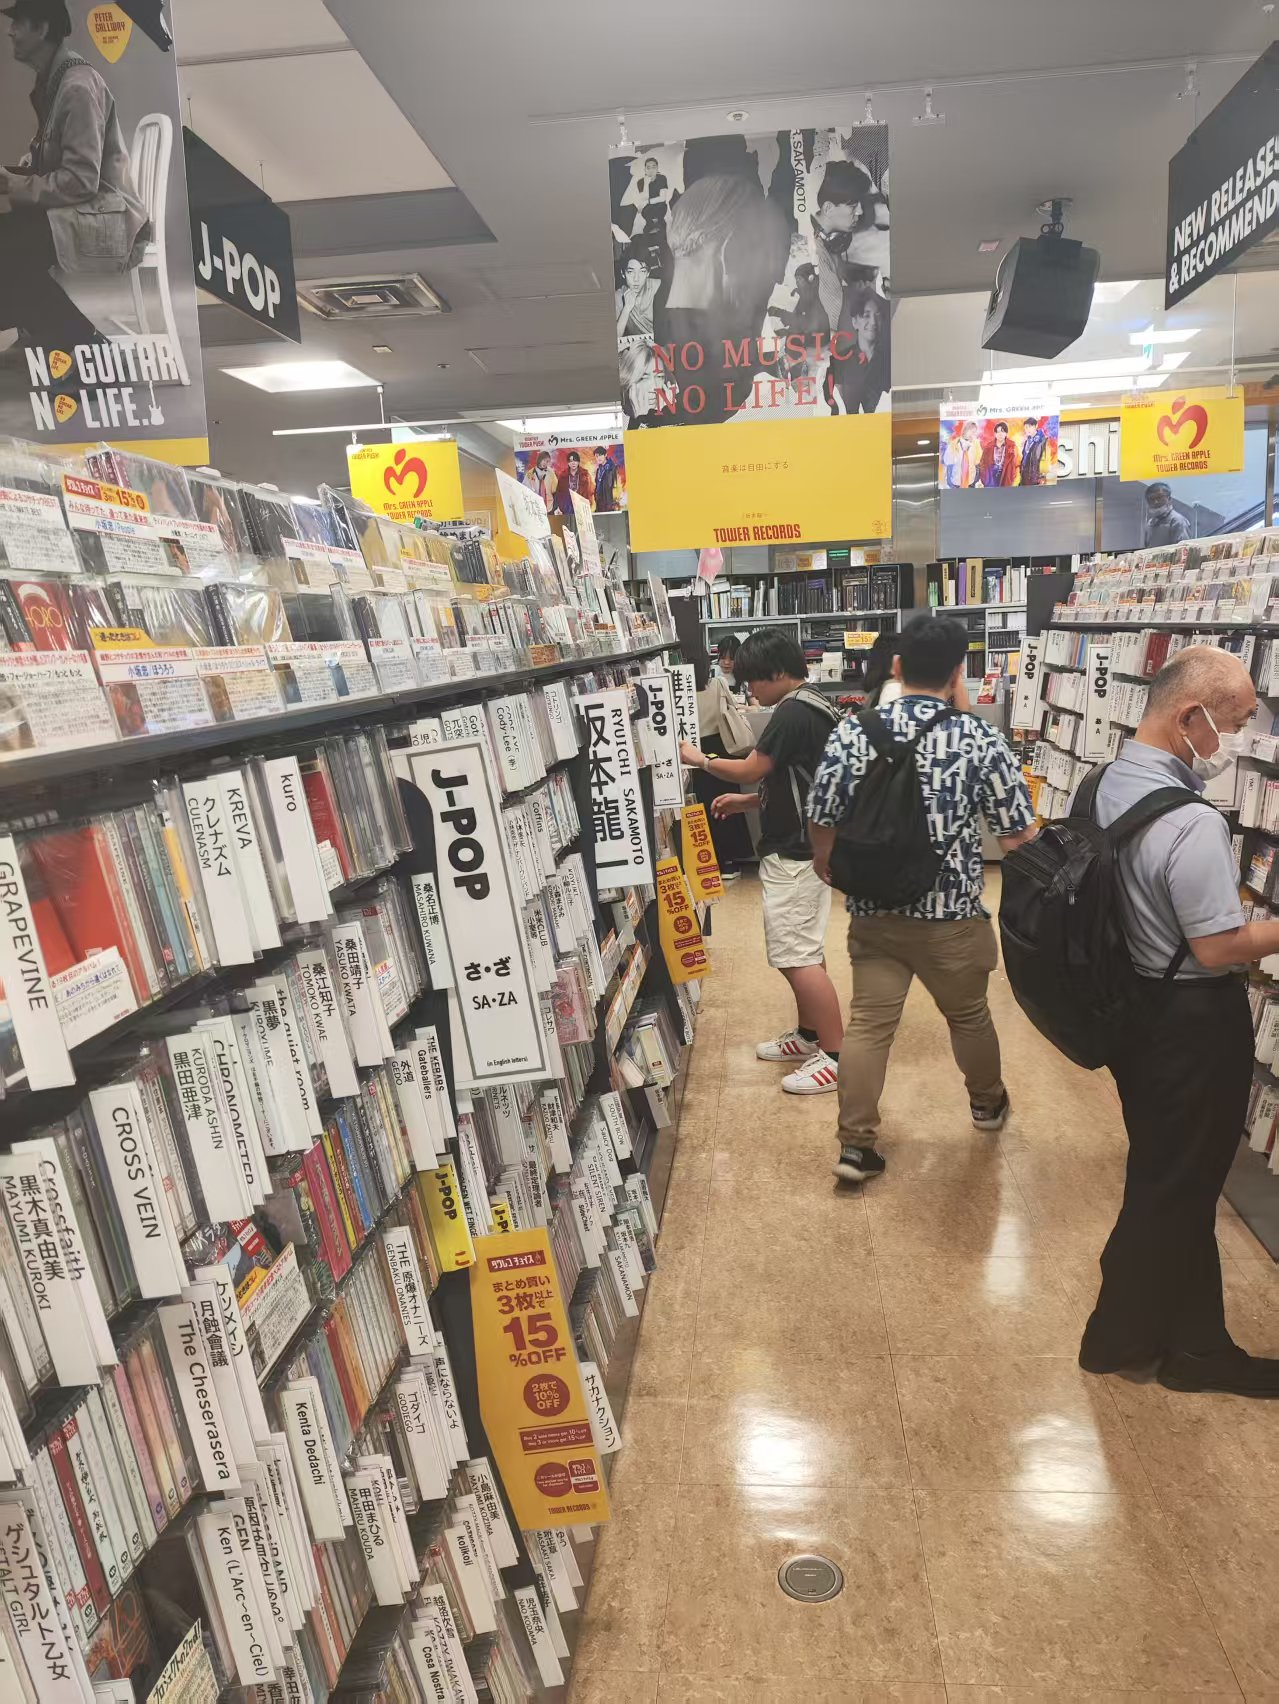
\includegraphics[height=6cm]{../source/pic5.png}

\vspace{10pt}

\textbf{其他名称}:无

\vspace{10pt}

\textbf{用途}:MdOI R2 C

\vspace{10pt}

\textbf{提交方式}:Luogu P6381

\vspace{10pt}

\textbf{难度}:$4/10$

\vspace{10pt}

\textbf{Tag}:图论,数论

\end{center}
\vspace*{\fill}

\newpage

\section*{背景}

原本只有一个“完美数对”的 idea,然后感觉太简单了就和 DAG 上的 DP 套了一下。

洛谷上的题目背景描述了几何冲刺最难 Demon 的变迁,当时的最难 Demon 是 The Golden,即下文的“金色遗迹”:

\begin{center}
超越音速的极限,不及瑰丽多变的极光;

微弱的脉冲,开拓原本一片混沌的天地;

沉郁的蓝缓缓闪动,史诗的红迎接巅峰;

血色的夕阳尽头,是将夜的星辰;

夜半的满天星空,也会被来自地狱的硝烟掩盖;

炽红炼狱消逝,只金色遗迹永存。

在这里等待着每一位的,都是一段艰苦而璀璨的旅程。
\end{center}

\section*{题目描述}

若正整数 $a$ 与 $b$ 满足:

\begin{itemize}
\item $a$ 与 $b$ 的积是一个正整数的 $k$ 次方,即存在正整数 $c$ 使得 $ab=c^k$。
\end{itemize}

那么我们称 $(a,b)$ 为一组\textbf{完美数对}。

有一个包含 $n$ 个结点和 $m$ 条边的\textbf{有向无环图},这张图中的每条边都有权值和长度两个属性。

如果一条路径 $P$ 满足\textbf{以下条件之一},则称其为一条\textbf{完美路径}:

\begin{itemize}
\item $P$ 中仅包含一条边。

\item $P$ 从其起点开始依次为 $e_1, e_2, e_3, \ldots e_p$ 这 $p\ (p\ge 2)$ 条边,对于任意的 $1\leq i\leq p-1$,$e_i$ 的权值和 $e_{i+1}$ 的权值组成完美数对。
\end{itemize}

你需要求出图中最长完美路径的长度,一条路径的长度定义为这条路径上所有边的长度之和。

\section*{数据范围}

$1\leq n\leq 10^5,\ 1\leq m\leq 2\times 10^5,\ 1\leq k\leq 10,\ 1\leq u,v\leq n,\ 1\leq w\leq 10^5,\ 1\leq l\leq 10^4$

\newpage

\vspace*{\fill}
\begin{center}

\section{\textcolor{red}{Match}}

\subsection*{2020.7}

\vspace{10pt}

\textbf{其他名称}:无

\vspace{10pt}

\textbf{用途}:被卖了(流泪)

\vspace{10pt}

\textbf{提交方式}:无

\vspace{10pt}

\textbf{难度}:$8/10$

\vspace{10pt}

\textbf{Tag}:字符串

\end{center}
\vspace*{\fill}

\newpage

\section*{背景}

讲件很有意思的事情,2020 年 7 月我把这题卖给神秘人,2022 年 7 月学弟在 ZROI 上做到了这道题,据说那场的出题人是一个之前的国家队(?)。谢谢你,蒙古人。

本题还有一个对偶版本没出,不过需要 FFT,不知道啥时候有机会出。

\section*{题目描述}

非公开

\newpage

\vspace*{\fill}
\begin{center}

\section{\textcolor{red}{Tom \& Jerry}}

\subsection*{2020.9}

\vspace{10pt}

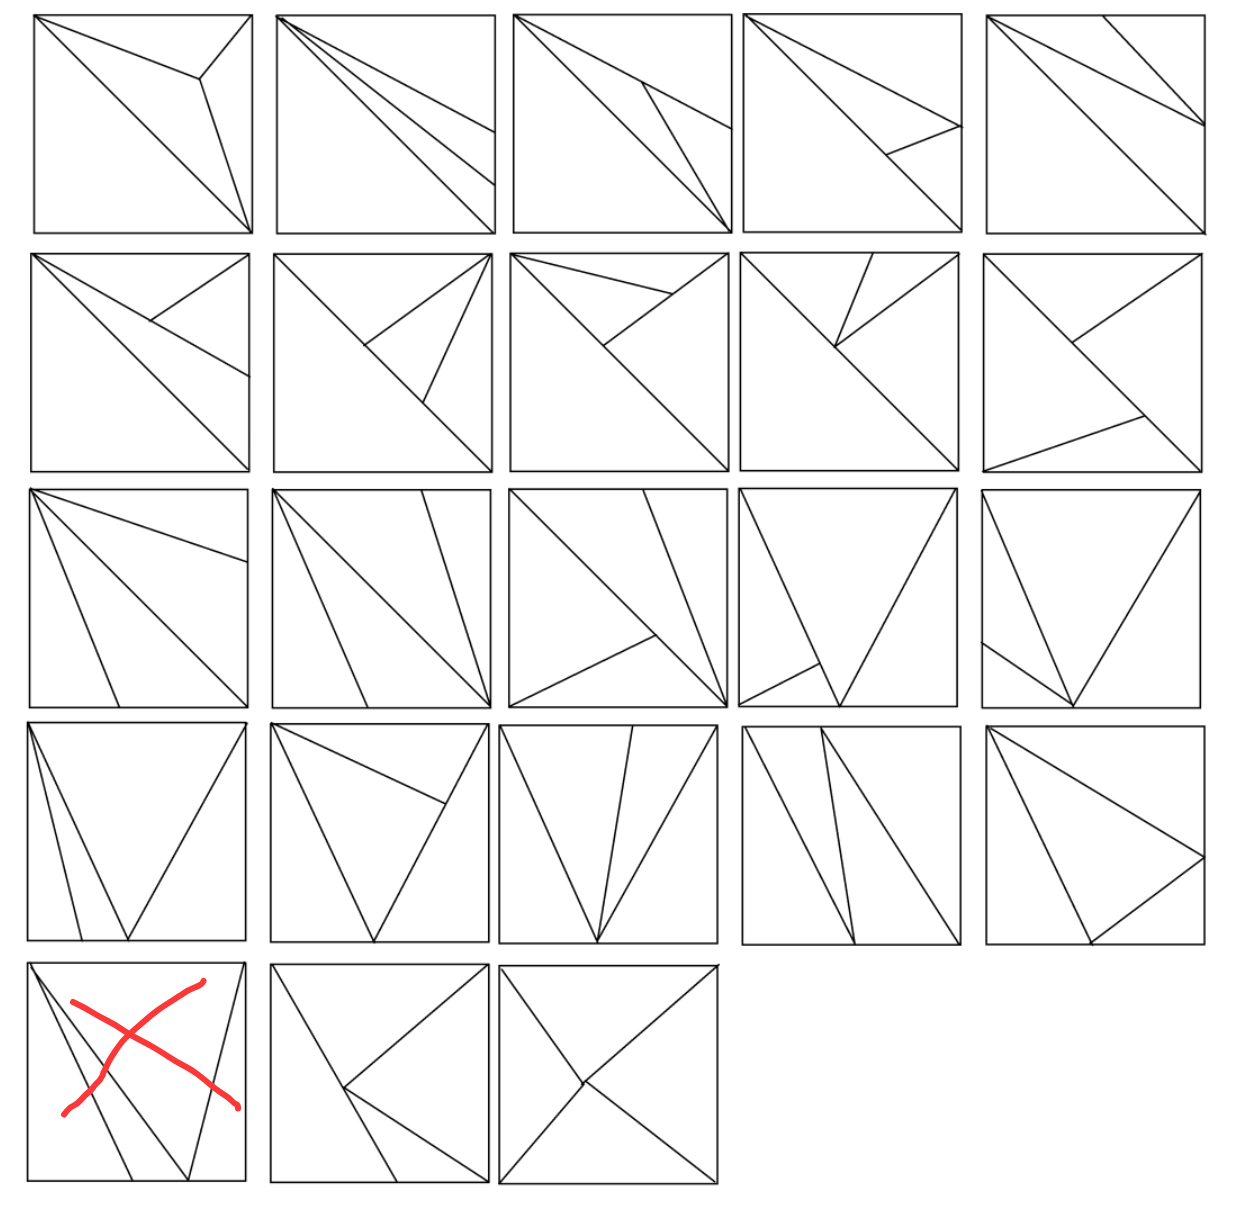
\includegraphics[height=6cm]{../source/pic1.png}

\vspace{10pt}

\textbf{其他名称}:Tom and Jerry

\vspace{10pt}

\textbf{用途}:联测 / 2020 集训队作业自选题

\vspace{10pt}

\textbf{提交方式}:Luogu P7353 / LOJ 3406

\vspace{10pt}

\textbf{难度}:$8/10$

\vspace{10pt}

\textbf{Tag}:图论,DP

\end{center}
\vspace*{\fill}

\newpage

\section*{背景}

第一次出的联测题,不过可能难了一点所以最高分只有十几分。后来集训队作业布置之后就把这题挂到集训队作业 OJ 上,当成自选题了,后来被搬到了洛谷和 LOJ。

\section*{题目描述}

给定一张包含 $n$ 个顶点和 $m$ 条边的\textbf{无向连通图},Tom 和 Jerry 在图上进行了 $q$ 次追逐游戏。

在第 $i$ 次游戏中,Tom 一开始位于顶点 $a_i$,而 Jerry 一开始位于顶点 $b_i$(双方任何时候都知道自己和对方的位置),追逐规则如下:

\begin{itemize}
\item Jerry 和 Tom 交替行动,Jerry 先行动。

\item Jerry 每次行动可以通过无向图中的\textbf{任意多条边}(可以选择不移动),但是在移动过程中不能经过 Tom 当前所在的结点,否则就会被抓住。

\item Tom 每次行动只能通过无向图中的\textbf{至多一条边}(可以选择不移动)。

\item 如果 Tom 在一次行动后到达了 Jerry 的位置,那么 Tom 胜利。
\end{itemize}

Tom 尽量想要胜利,而 Jerry 会尽量阻止 Tom 胜利。

现在你需要对于每一局游戏,求出 Tom 是否一定能在有限次行动内获胜。

\section*{数据范围}

$1\leq n,m,q\leq 10^5$,$1\leq x,y,a,b\leq n$,$a_i\ne b_i$

保证给出的无向图连通,且不含重边和自环。

\newpage

\vspace*{\fill}
\begin{center}

\section{恭喜你发现签到题}

\subsection*{2020.11}

\vspace{10pt}

\includegraphics[height=2.4cm]{../source/pic8.png}

\vspace{10pt}

\textbf{其他名称}:无

\vspace{10pt}

\textbf{用途}:联测

\vspace{10pt}

\textbf{提交方式}:无(不过可以做一下 AGC 044 D)

\vspace{10pt}

\textbf{难度}:$4/10$

\vspace{10pt}

\textbf{Tag}:字符串,交互

\end{center}
\vspace*{\fill}

\newpage

\section*{背景}

出到 WC 联测,结果好像十几分钟内就被风口浪尖的集训队员给过了。

后记:详见上一页图片。

\section*{题目描述}

\textbf{本题为交互题。}

有一个未知的字符串 $S$,它的字符集是 $\text{\{a,b,c\}}$,它的长度在 $[L,R]$ 中,其中 $L,R$ 是给定的常数。

为了猜出这个字符串,你可以做若干次询问,每次询问中:

\begin{itemize}
\item {你需要给出一个\textbf{长度不超过 $R$ 的,字符集为 $\text{\{a,b,c\}}$ 的}字符串 $T$;}

\item {交互库会返回:$T$ 是否是 $S$ 的\textbf{子序列}(不必连续)。}
\end{itemize}

设 $S$ 的\textbf{实际长度}为 $n$,你需要在 $\lfloor k\times n\rfloor$ 次询问以内得到 $S$,其中 $k$ 是给定的常数。

\section*{数据范围}

最后子任务:$L=2000,\ R=4000,\ k=1.7$

\newpage

\vspace*{\fill}
\begin{center}

\section{记忆}

\subsection*{2020.?}

\vspace{10pt}

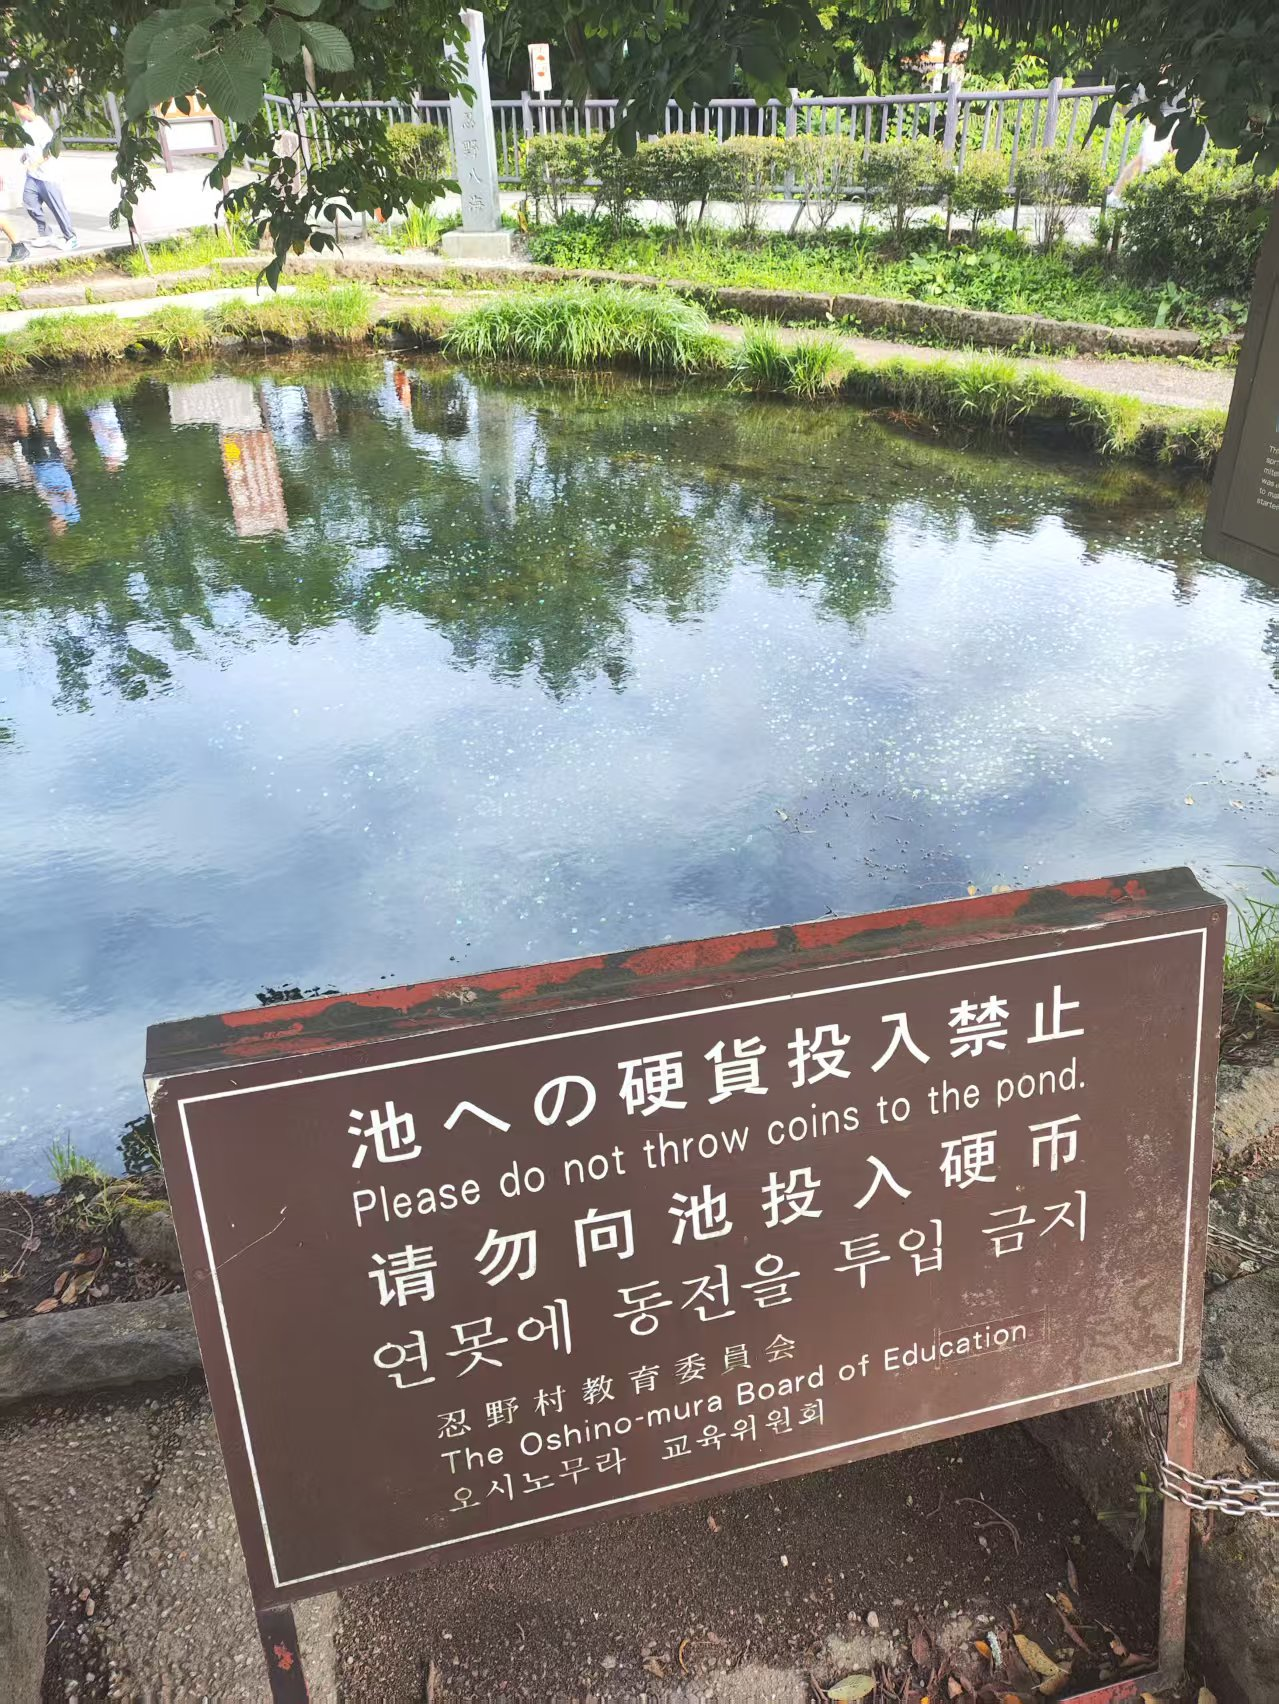
\includegraphics[height=5cm]{../source/pic7.png}

\vspace{10pt}

\textbf{其他名称}:无

\vspace{10pt}

\textbf{用途}:Rochine Round 3 E

\vspace{10pt}

\textbf{提交方式}:Luogu P6864

\vspace{10pt}

\textbf{难度}:$5/10$

\vspace{10pt}

\textbf{Tag}:数据结构

\end{center}
\vspace*{\fill}

\newpage

\section*{背景}

有一天,一个叫 Feecle6418 的人在洛谷上征题,正好 MdOI 题都够了,我就把这题给他了。

原背景:小 W 想写一个关于记忆的题目背景,但是他忘记了。

\section*{题目描述}

有一个括号串 $S$,一开始 $S$ 中只包含一对括号(即初始的 $S$ 为 $\texttt{()}$),接下来有 $n$ 个操作,操作分为三种:

1. 在当前 $S$ 的末尾加一对括号(即 $S$ 变为 $S\texttt{()}$);

2. 在当前 $S$ 的最外面加一对括号(即 $S$ 变为 $\texttt{(}S\texttt{)}$);

3. 取消第 $x$ 个操作,即去除第 $x$ 个操作造成过的\textbf{一切影响}(例如,如果第 $x$ 个操作也是取消操作,且取消了第 $y$ 个操作,那么当前操作的实质就是恢复了第 $y$ 个操作的作用效果)。

每次操作后,你需要输出 $S$ 的能够括号匹配的非空子串(子串要求连续)个数。

一个括号串能够括号匹配,当且仅当其左右括号数量相等,且任意一个前缀中左括号数量不少于右括号数量。

\section*{数据范围}

$1\leq n\leq 2\times 10^5,\ op\in \{1,2,3\},\ 1\leq x\leq n$

一个操作在形式上最多只会被取消一次(即所有 $x$ 互不相同)。

\newpage

\vspace*{\fill}
\begin{center}

\section{切蛋糕}

\subsection*{2021.3}

\vspace{10pt}

\includegraphics[height=2cm]{../source/pic14.png}\footnote{图片由 uwagjaynoi 绘制。}

\vspace{10pt}

\textbf{其他名称}:无

\vspace{10pt}

\textbf{用途}:NOI Online 2021 入门组 T1

\vspace{10pt}

\textbf{提交方式}:Luogu P7471

\vspace{10pt}

\textbf{难度}:$1/10$

\vspace{10pt}

\textbf{Tag}:无

\end{center}
\vspace*{\fill}

\newpage

\section*{背景}

很好一个签到题。

\section*{题目描述}

Alice,Bob 和 Cindy 三个好朋友得到了一个圆形蛋糕,他们打算分享并吃完这个蛋糕。

每人分别有一个需求量 $a,b,c$,现在请你帮他们切蛋糕,规则如下:

\begin{itemize}
\item 每次切蛋糕可以选择蛋糕的任意一条直径,沿这条直径切一刀(注意切完后不会立刻将蛋糕分成两部分);

\item 设你一共切了 $n$ 刀,那么你将得到 $2n$ 个扇形(特别地,切了 $0$ 刀被认为是有一个扇形,即整个圆),将这些扇形分配给 Alice,Bob 和 Cindy,要求每个扇形只能完整地分给一个人,且三人分到的面积比需要为 $a:b:c$(不保证是最简比例,且如果 $a,b,c$ 中某个数为 $0$,表示那个人不吃蛋糕)。
\end{itemize}

为了完成这个任务,你至少需要切几刀?

本题单个测试点包含 $T$ 组数据。

\section*{数据范围}

$1\leq T\leq 10^4,\ 0\leq a,b,c\leq 10^8,\ a+b+c>0$

\newpage

\vspace*{\fill}
\begin{center}

\section{吃豆人}

\subsection*{2021.3}

\vspace{10pt}

\includegraphics[height=8cm]{../source/pic15.png}\footnote{图片由 uwagjaynoi 绘制。}

\vspace{10pt}

\textbf{其他名称}:无

\vspace{10pt}

\textbf{用途}:NOI Online 2021 入门组 T2

\vspace{10pt}

\textbf{提交方式}:Luogu P7472

\vspace{10pt}

\textbf{难度}:$2/10$

\vspace{10pt}

\textbf{Tag}:无

\end{center}
\vspace*{\fill}

\newpage

\section*{背景}

我没玩过吃豆人,感觉不如糖豆人。

\section*{题目描述}

有一个 $n$ 行 $n$ 列的正方形点阵,左上角点坐标为 $(1,1)$,右下角点坐标为 $(n,n)$。

点阵中每个整点上都有数量不一的豆子,坐标为 $(i,j)$ 的点上有 $a_{i,j}$ 个豆子。

你可以放置吃豆人,可以将点阵中任意的整点作为吃豆人的初始位置,再给定左上、左下、右上、右下之一作为吃豆人的初始方向。

吃豆人会不断沿初始方向行进,吃光遇到的所有豆子,直到碰到点阵的边界,此时:

\begin{itemize}
\item 如果吃豆人处于正方形点阵四个角之一的位置,那么就会停止行动;

\item 否则,吃豆人的行进路线将以这条边界为镜面发生反射。
\end{itemize}

现在,你需要放置两个吃豆人,求两个吃豆人最多共能吃到多少个豆子?注意同一个豆子只能被吃一次。

\section*{数据范围}

$2\leq n\leq 10^3,\ 0\leq a_{i,j}\leq 10^3$

\newpage

\vspace*{\fill}
\begin{center}

\section{重力球}

\subsection*{2021.3}

\vspace{10pt}

\includegraphics[height=8cm]{../source/pic16.png}\footnote{图片由 uwagjaynoi 绘制。}

\vspace{10pt}

\textbf{其他名称}:无

\vspace{10pt}

\textbf{用途}:NOI Online 2021 入门组 T3

\vspace{10pt}

\textbf{提交方式}:Luogu P7473

\vspace{10pt}

\textbf{难度}:$4/10$

\vspace{10pt}

\textbf{Tag}:无

\end{center}
\vspace*{\fill}

\newpage

\section*{背景}

本题灵感是来自几何冲刺中的 Ball 模式。

感谢 uwagjaynoi 用几何画板帮我画的这三题的配图。

\section*{题目描述}

“重力球”游戏在一块 $n\times n$ 的正方形区域中进行,称从上往下第 $i$ 行,从左往右第 $j$ 列的位置为 $(i,j)$。

正方形区域中存在 $m$ 个障碍,第 $i$ 个障碍占据位置 $(x_i,y_i)$,此外,正方形区域的边界外都是障碍。

现在有两个小球,位置分别是 $(a,b)$ 和 $(c,d)$,在游戏中你可以进行如下操作:

\begin{itemize}
\item 指定上、下、左、右中的一个方向,将重力方向“切换”为这个方向,即两个小球会同时向这个方向移动,直到碰到障碍。
\end{itemize}

你要用最少的操作次数使得两个小球到达同一个位置。

现有 $q$ 局游戏,每局游戏中只有小球的初始位置不同,而障碍位置是不变的,你需要对每局游戏都求出最小操作次数,或报告无解。

\section*{数据范围}

$1\leq n,m\leq 250,\ 1\leq q\leq 10^5$

\newpage

\vspace*{\fill}
\begin{center}

\section{远古档案馆}

\subsection*{2021.7}

\vspace{10pt}

\includegraphics[height=6cm]{../source/pic10.png}

\vspace{10pt}

\textbf{其他名称}:无

\vspace{10pt}

\textbf{用途}:ix35 月赛 I A

\vspace{10pt}

\textbf{提交方式}:Luogu P7724

\vspace{10pt}

\textbf{难度}:$1/10$

\vspace{10pt}

\textbf{Tag}:无

\end{center}
\vspace*{\fill}

\newpage

\section*{背景}

原本的 A 题是另一个题,但被 zjc 查重了(奥林匹克五子棋),所以换成了这题。本题题目名称来自饥荒联机版 DLC 旧神归来,远古档案馆是洞穴中的一个区域,当然请注意远古档案馆的解谜与本题的描述是不同的。原背景:

为了揭开月光能量背后的秘密,你来到了地下的远古档案馆。

远古一族的秘密与遗忘的知识悉数贮藏于这片被尘封的迷宫中,你能成功解谜,获知远古的知识吗?

\section*{题目描述}

远古档案馆的中心是一个解谜:

\begin{itemize}
\item 有一个 $2\times 2$ 的网格,每个格子中要么有一个正整数,要么是空的;

\item 你可以进行若干次操作:每次操作中,你选择一个\textbf{有正整数的格子}和一个\textbf{与之相邻的空格子},将正整数移到那个空格子中;

\item 给定网格的初始状态和最终状态,保证初始状态和最终状态中包含的正整数个数相同(设为 $k$ 个),且它们就是前 $k$ 个不同的正整数,问是否可以通过有限次操作从初始状态到达最终状态?
\end{itemize}

只有完成解谜,才能获得遗忘的知识,因此你希望尽快解决这个问题。

\textbf{注意:网格中可能没有正整数,也可能没有空格。}

\section*{数据范围}

所有数据符合题目描述所述。

\newpage

\vspace*{\fill}
\begin{center}

\section{珍珠帝王蟹}

\subsection*{2021.7}

\vspace{10pt}

\includegraphics[height=6cm]{../source/pic11.png}

\vspace{10pt}

\textbf{其他名称}:幸运

\vspace{10pt}

\textbf{用途}:ix35 月赛 I B

\vspace{10pt}

\textbf{提交方式}:Luogu P7725

\vspace{10pt}

\textbf{难度}:$2/10$

\vspace{10pt}

\textbf{Tag}:无

\end{center}
\vspace*{\fill}

\newpage

\section*{背景}

本题题目名称来自饥荒联机版 DLC 旧神归来,帝王蟹是海上的一个 boss,可以镶嵌珍珠使其得到巨大强化,称为珍珠帝王蟹,当然请注意强化的规则和本题的描述是不同的。原背景:

在一次航程中,你偶然发现了被一片礁石环绕的帝王蟹,被月岛能量侵蚀的它又与月光有着怎样的联系呢?似乎只有击败它才能见分晓。

\section*{题目描述}

帝王蟹可以通过镶嵌宝石触发战斗,不同的宝石效果不同,但奇特的是,镶嵌宝石的顺序有时也会影响它的强度。

帝王蟹有一个初始为 $0$ 的强度值,每个宝石有属性 $op$ 和 $v$,表示:

\begin{itemize}
\item 若 $op$ 为 $\texttt{+}$,则镶嵌后帝王蟹的强度值将会加上 $v$;

\item 若 $op$ 为 $\texttt{*}$,则镶嵌后帝王蟹的强度值将会乘上 $v$。
\end{itemize}

由于宝石的效果十分奇异,所以 $v$ 可能是负数。

作为一个有挑战精神的冒险者,你希望采取某种镶嵌方式,将\textbf{每个宝石}都镶嵌\textbf{恰好一遍},且使得帝王蟹的强度值最大。

你只需要输出最大的强度值对 $998244353$ 取模的结果。

\section*{数据范围}

$1\leq n\leq 10^5,\ 2\leq |v|\leq 10^6$

\newpage

\vspace*{\fill}
\begin{center}

\section{天体探测仪}

\subsection*{2021.7}

\vspace{10pt}

\textbf{其他名称}:无

\vspace{10pt}

\textbf{用途}:ix35 月赛 I C

\vspace{10pt}

\textbf{提交方式}:Luogu P7726

\vspace{10pt}

\textbf{难度}:$4/10$

\vspace{10pt}

\textbf{Tag}:构造

\end{center}
\vspace*{\fill}

\newpage

\section*{背景}

本题题目名称来自饥荒联机版 DLC 旧神归来,天体探测仪是由在远古档案馆中知识蒸馏得到的蓝图建造的仪器。原背景:

通过远古档案馆的探索,你成功制出了天体探测仪,你需要用它发现潜藏的天体科技。

\section*{题目描述}

想要找到天体科技,你需要先得到一串天体密码——它是一个 $1 \sim n$ 的\textbf{排列}。天体探测仪允许对于给定的长度 $l$,返回密码中一个长度为 $l$ 的\textbf{区间的最小值}。

不幸的是,所有长度为 $l$ 的区间最小值混在了一起,你得到的只是 $n$ 个\textbf{可重集合} $S_1,\ldots,S_n$,其中:

\begin{itemize}
\item $S_i$ 表示所有长度为 $i$ 的区间最小值构成的可重集合。
\end{itemize}

你需要根据这些 $S_i$,还原出一种可能的天体密码,保证至少存在一种正确的天体密码。

\section*{数据范围}

$2\leq n\leq 800$

\newpage

\vspace*{\fill}
\begin{center}

\section{风暴之眼}

\subsection*{2021.7}

\vspace{10pt}

\includegraphics[height=6cm]{../source/pic12.png}

\vspace{10pt}

\textbf{其他名称}:Headmaster III

\vspace{10pt}

\textbf{用途}:ix35 月赛 I D

\vspace{10pt}

\textbf{提交方式}:Luogu P7727

\vspace{10pt}

\textbf{难度}:$5/10$

\vspace{10pt}

\textbf{Tag}:DP

\end{center}
\vspace*{\fill}

\newpage

\section*{背景}

本题题目名称来自饥荒联机版 DLC 旧神归来,风暴之眼是建造未完成的实验后产生的事件。原背景:

通过月岛,帝王蟹和天体探测仪,你成功拼合了三个天体科技,接下来你要做的,就是来到风暴之眼的中心,准备那个神秘实验的最后一步。

最终的真相近在咫尺,你能否成功通过这场考验呢?

\section*{题目描述}

天体风暴中的气象瞬息万变。

风暴中的道路构成一棵 $n$ 个结点的\textbf{无根树},第 $i$ 个结点有初始权值 $w_i$($w_i$ 为 $0$ 或 $1$)和类型 $t_i$。

结点的类型分为两种:$\texttt{AND}$ 型结点和 $\texttt{OR}$ 型结点。

对于 $\texttt{AND}$ 型结点,每一秒结束后它的权值将变为它与它所有邻居上一秒权值的 $\texttt{AND}$ 和;

对于 $\texttt{OR}$ 型结点,每一秒结束后它的权值将变为它与它所有邻居上一秒权值的 $\texttt{OR}$ 和。

现在,已知从某一时刻起,所有结点的权值都不再发生任何变化,将此时点 $i$ 的权值称为 $a_i$。

现不知每个点的初始权值和类型,只知道最终每个点的权值 $a_i$,求出有多少种可能的初始权值和类型的组合,答案对 $998244353$ 取模。

\section*{数据范围}

$2\leq n\leq 2\times 10^5,\ 1\leq x,y\leq n,\ a_i\in \{0,1\}$

\newpage

\vspace*{\fill}
\begin{center}

\section{\textcolor{red}{旧神归来}}

\subsection*{2021.7}

\vspace{10pt}

\includegraphics[height=6cm]{../source/pic13.png}

\vspace{10pt}

\textbf{其他名称}:钞现实树

\vspace{10pt}

\textbf{用途}:ix35 月赛 I E

\vspace{10pt}

\textbf{提交方式}:Luogu P7728

\vspace{10pt}

\textbf{难度}:$8/10$

\vspace{10pt}

\textbf{Tag}:计数

\end{center}
\vspace*{\fill}

\newpage

\section*{背景}

本题题目名称来自饥荒联机版 DLC 旧神归来。原背景:

随着虚影与暗影的决战、月岛祭坛的完工、天体风暴的出现、天界捍卫者的到来,一切月球与远古的秘密仿佛已经行至终局。

旧神即将归来!

\section*{题目描述}

月岛上的一棵普通的树在月光侵蚀的影响下不断生长,随着月面风暴的来临变得更加无限制。

具体地,生长规则如下:

\begin{itemize}
\item 初始有一棵包含 $n$ 个结点的以 $1$ 为根的\textbf{有根树} $T_0$;

\item 在第 $i$ 天,树将从 $T_{i-1}$ 生长为 $T_i$,生长规则为:令 $v$ 是 $T_{i-1}$ 中\textbf{深度最小的叶结点}(若有多个则任意选择一个),以 $v$ 这个点替换成 $T_{i-1}$ 本身。
\end{itemize}

本题中一个结点的深度定义为它到根结点的简单路径所经过的\textbf{边数},注意这可能与常规定义不同。

除了面对天界捍卫者,对于环境效应的估计也是重要的,所以你要计算:

\begin{itemize}
\item 对于每个整数 $d\in [1,m]$,求出 $S_d$ 表示最小的天数,满足 $T_{S_d}$ 中深度最小的叶结点深度\textbf{大于} $d$。
\end{itemize}

答案对 $998244353$ 取模。

\section*{数据范围}

$2\leq n,m\leq 10^5$

\newpage

\vspace*{\fill}
\begin{center}

\section{线段树}

\subsection*{2021.7}

\vspace{10pt}

\includegraphics[height=4cm]{../source/pic18.png}

\vspace{10pt}

\textbf{其他名称}:无

\vspace{10pt}

\textbf{用途}:联测

\vspace{10pt}

\textbf{提交方式}:无

\vspace{10pt}

\textbf{难度}:$4/10$

\vspace{10pt}

\textbf{Tag}:交互

\end{center}
\vspace*{\fill}

\newpage

\section*{背景}

写完 NOI 一轮复习线段树那部分之后出的随堂练习题,好像有点简单。

\section*{题目描述}

找不到了,大意就是有一棵 $[1,n]$ 的广义线段树,每次可以问 $[l,r]$ 的区间定位数,要在 $2\times n-1$ 次操作内确定结构。

\section*{数据范围}

找不到了,大概是 $n\leq 10^5$。

\newpage

\vspace*{\fill}
\begin{center}

\section{Origami}

\subsection*{2021.10}

\vspace{10pt}

\includegraphics[height=5cm]{../source/pic21.png}

\vspace{10pt}

\textbf{其他名称}:无

\vspace{10pt}

\textbf{用途}:神秘比赛 T1

\vspace{10pt}

\textbf{提交方式}:无

\vspace{10pt}

\textbf{难度}:$2/10$

\vspace{10pt}

\textbf{Tag}:无

\end{center}
\vspace*{\fill}

\newpage

\section*{背景}

关于题目名称:指鸢一折纸,这里借做序数词。

\section*{题目描述}

给定长度为 $n$ 的字符串 $A_0$ 和长度为 $m$ 的字符串 $B_0$,它们都只包含大小写字母。对于任意整数 $i\ge 1$,令 $A_i$ 是由 $A_{i-1}$ 与 $B_{i-1}$ 拼接而成的字符串,$B_i$ 是由 $B_{i-1}$ 与 $A_{i-1}$ 拼接而成的字符串。

有 $T$ 个询问,每个询问给定 $x$,你需要输出 $A_{935}$ 中的第 $x$ 个字符是什么。

\section*{数据范围}

$1\leq n,m,T\leq 10^4,\ 1\leq x\leq 10^{15}$

\newpage

\vspace*{\fill}
\begin{center}

\section{Nia}

\subsection*{2021.10}

\vspace{10pt}

\includegraphics[height=6cm]{../source/pic22.png}

\vspace{10pt}

\textbf{其他名称}:无

\vspace{10pt}

\textbf{用途}:神秘比赛 T2

\vspace{10pt}

\textbf{提交方式}:无

\vspace{10pt}

\textbf{难度}:$4/10$

\vspace{10pt}

\textbf{Tag}:图论

\end{center}
\vspace*{\fill}

\newpage

\section*{背景}

关于题目名称:指本条二亚,这里借做序数词。

\section*{题目描述}

给定整数 $n$,设 $M=\dfrac{n(n-1)}{2}$,显然 $n$ 个点的完全图包含 $M$ 条边。

现给定一个包含 $n$ 个点的树 $T$,点编号为 $1,\ldots,n$,边有边权,保证边权是 $[1,M]$ 中互不相同的整数。

你需要在树的基础上添加 $M-n+1$ 条边,形成一个边有权值的完全图 $G$,并且满足:

\begin{itemize}
\item $T$ 是 $G$ 的一棵最小生成树;

\item $G$ 中所有边的边权是 $[1,M]$ 中互不相同的整数。
\end{itemize}

请你首先求出符合条件的 $G$ 的数量,答案对 $10^9+7$ 取模。

此外,如果存在符合条件的 $G$,则你需要再构造出一种这样的 $G$。

\section*{数据范围}

$1\leq n\leq 800$

\newpage

\vspace*{\fill}
\begin{center}

\section{Kurumi}

\subsection*{2021.10}

\vspace{10pt}

\includegraphics[height=6cm]{../source/pic23.png}

\vspace{10pt}

\textbf{其他名称}:ix100

\vspace{10pt}

\textbf{用途}:神秘比赛 T3

\vspace{10pt}

\textbf{提交方式}:无

\vspace{10pt}

\textbf{难度}:$5/10$

\vspace{10pt}

\textbf{Tag}:字符串,计数

\end{center}
\vspace*{\fill}

\newpage

\section*{背景}

根据脑力延申出的一道题。

关于题目名称:指时崎狂三,这里借做序数词。

\section*{题目描述}

给定 $n$ 个数字串 $S_1,\ldots,S_n$,每个串的长度都为 $m$。

然而,现在每个字符串内部的字符顺序都可能出现随机的调换,例如若 $S=\texttt{012}$,那么调换后 $S_i$ 会等概率随机成为 $\texttt{012},\texttt{021},\texttt{102},\texttt{120},\texttt{201},\texttt{210}$ 中的一种。

现要把调换后的 $n$ 个数字串全部插入一棵字典树中(调换的结果是等概率随机的),问这个字典树结点数量的期望是多少,答案对 $998244353$ 取模。

\section*{数据范围}

$\xout{1\leq n\leq 100}$

$1\leq n\leq 10,\ 1\leq m\leq 100$

\newpage

\vspace*{\fill}
\begin{center}

\section{\textcolor{red}{Yoshino}}

\subsection*{2021.10}

\vspace{10pt}

\includegraphics[height=6cm]{../source/pic24.png}

\vspace{10pt}

\textbf{其他名称}:无

\vspace{10pt}

\textbf{用途}:神秘比赛 T4

\vspace{10pt}

\textbf{提交方式}:无

\vspace{10pt}

\textbf{难度}:$8/10$

\vspace{10pt}

\textbf{Tag}:数据结构

\end{center}
\vspace*{\fill}

\newpage

\section*{背景}

我也许以后会把这几道题公开到某个地方。

灵感来源是几何冲刺中的 Wave。

关于题目名称:指冰芽川四糸乃,这里借做序数词。

\section*{题目描述}

在平面直角坐标系中,我们称竖直线 $x=-10^{935}$ 和 $x=10^{935}$ 之间的区域为“场地”。

有一个 Wave 在场地中飞行,规则如下:

\begin{itemize}
\item Wave 从场地最左侧(竖直线 $x=-10^{935}$ 上)任意一点出发,到达最右侧(竖直线 $x=10^{935}$ 上)任意一点结束;

\item Wave 在水平方向的速度始终为 $1$,而任意时刻竖直方向速度可以为 $-1$ 或 $1$,也就是说,Wave 始终朝右上或右下方向飞行,注意 Wave 可以在任意时刻改变方向,也就是说一条近似于水平直线的运动轨迹也是可能出现的;

\item 场地上有 $m$ 个障碍,第 $i$ 个障碍是一条竖直线段,下端点为 $(x_i,y_{i,0})$,上端点为 $(x_i,y_{i,1})$,Wave 在飞行过程中不能触碰障碍(包括端点)。
\end{itemize}

现在请问:Wave 在一次完整飞行过程中一定无法经过的区域面积是多少?

\section*{数据范围}

$1\leq m\leq 2\times 10^5,\ 0\leq x_i\leq 10^5,\ 0\leq y_{i,0}< y_{i,1}\leq 10^5$


$y_{i,1}-y_{i,0}$ 为偶数。

\newpage

\vspace*{\fill}
\begin{center}

\section{Speike \& Tom}

\subsection*{2021.10}

\vspace{10pt}

\includegraphics[height=6cm]{../source/pic17.png}

\vspace{10pt}

\textbf{其他名称}:Speike and Tom

\vspace{10pt}

\textbf{用途}:2021 集训队互测

\vspace{10pt}

\textbf{提交方式}:LOJ 3638

\vspace{10pt}

\textbf{难度}:$7/10$

\vspace{10pt}

\textbf{Tag}:数据结构

\end{center}
\vspace*{\fill}

\newpage

\section*{背景}

为了集训队互测出的一道题,但是有些臃肿了,不是很满意。

\section*{题目描述}

一次 Tom 准备用鞭炮炸 Jerry 的老鼠洞时,不小心炸到了 Speike 的狗窝。

后院的道路构成了一棵 $n$ 个点的\textbf{无向树},Speike 与 Tom 之间的追逐以如下方式展开:

\begin{itemize}
\item Tom 和 Speike 一开始分别在 $a,b$ 两个点;

\item Tom 和 Speike 轮流行动,Tom 先行;

\item 每次行动者可以选择不动,或是沿着一条边走到另一个端点;

\item 如果一次行动后到达了 Speike 和 Tom 处于同一位置则 Speike 胜。
\end{itemize}

以 Tom 的智商足够知道这个游戏他是必败的,所以他趁 Speike 没反应过来之前建立了 $m$ 条\textbf{额外边},这些额外边\textbf{只能被 Tom 经过,而不能被 Speike 经过}。

现在 Tom 想要知道,对于所有的 $n\times (n-1)$ 组可能的 $(a,b)\ (a\ne b)$,有多少组追逐中 Tom 有策略使得 Speike 永远无法获胜。

\section*{数据范围}

$1\leq n,m\leq 10^5,\ 1\leq x,y\leq n$

\newpage

\vspace*{\fill}
\begin{center}

\section{Matrix}

\subsection*{2021.?}

\vspace{10pt}

\textbf{其他名称}:Core

\vspace{10pt}

\textbf{用途}:联测

\vspace{10pt}

\textbf{提交方式}:无

\vspace{10pt}

\textbf{难度}:$7/10$

\vspace{10pt}

\textbf{Tag}:计数

\end{center}
\vspace*{\fill}

\newpage

\section*{背景}

比较早就出出来的一个题,原本也想放月赛,但有了另一个更好的 NTT 题,于是这个题就放联测了。

\section*{题目描述}

对于一个 $n\times m$ 的仅由 $0,1$ 构成的矩阵 $M$,一个 $1,\ldots,n$ 的排列 $p_{1\ldots n}$ 和一个 $1,\ldots,m$ 的排列 $q_{1\ldots m}$,设 $M'=f_M(p,q)$ 为一个 $n\times m$ 的仅由 $0,1$ 构成的矩阵,其中 $M'_{p_i,q_j}=M_{i,j}$。

如果 $f_M(p,q)=M$,那么我们称 $(M,p,q)$ 为一个核心。

对于给定的 $p$,求出使得 $(M,p,q)$ 为核心的 $(M,q)$ 的个数。

\section*{数据范围}

$1\leq n,m\leq 10^5$

\newpage

\vspace*{\fill}
\begin{center}

\section{氮}

\subsection*{2022.9}

\vspace{10pt}

\textbf{其他名称}:无题

\vspace{10pt}

\textbf{用途}:xmoj

\vspace{10pt}

\textbf{提交方式}:无

\vspace{10pt}

\textbf{难度}:$2/10$

\vspace{10pt}

\textbf{Tag}:DP

\end{center}
\vspace*{\fill}

\newpage

\section*{背景}

只是一个水题。

\section*{题目描述}

非公开

http://xmoj.tech/problem.php?id=6193

\newpage

\vspace*{\fill}
\begin{center}

\section{氧}

\subsection*{2022.9}

\vspace{10pt}

\textbf{其他名称}:无题其二 / Atlantis / 庐山游

\vspace{10pt}

\textbf{用途}:xmoj

\vspace{10pt}

\textbf{提交方式}:无

\vspace{10pt}

\textbf{难度}:$3/10$

\vspace{10pt}

\textbf{Tag}:图论

\end{center}
\vspace*{\fill}

\newpage

\section*{背景}

比较有意思的题,原本想放 MdOI R2,后来忘了是啥原因没放。

\section*{题目描述}

非公开

http://xmoj.tech/problem.php?id=6194

\newpage

\vspace*{\fill}
\begin{center}

\section{氟}

\subsection*{2022.9}

\vspace{10pt}

\includegraphics[height=3cm]{../source/pic20.png}

\vspace{10pt}

\textbf{其他名称}:Low Complexity Tree / Headmaster II

\vspace{10pt}

\textbf{用途}:xmoj

\vspace{10pt}

\textbf{提交方式}:无

\vspace{10pt}

\textbf{难度}:$5/10$

\vspace{10pt}

\textbf{Tag}:DP

\end{center}
\vspace*{\fill}

\newpage

\section*{背景}

曾第二个被用作 ix35 月赛 I D 的题,但由于之后有个更好的所以换了。

\section*{题目描述}

非公开

http://xmoj.tech/problem.php?id=6195

\newpage

\vspace*{\fill}
\begin{center}

\section{暗物质}

\subsection*{2022.9}

\vspace{10pt}

\includegraphics[height=6cm]{../source/pic25.png}

\vspace{10pt}

\textbf{其他名称}:Pow

\vspace{10pt}

\textbf{用途}:ZROI

\vspace{10pt}

\textbf{提交方式}:无

\vspace{10pt}

\textbf{难度}:$1/10$

\vspace{10pt}

\textbf{Tag}:无

\end{center}
\vspace*{\fill}

\newpage

\section*{背景}

只是一个签到题。

题目名称出自星之卡比系列暗物质家族的真暗物质。

\section*{题目描述}

非公开

http://www.zhengruioi.com/problem/2345

\newpage

\vspace*{\fill}
\begin{center}

\section{零}

\subsection*{2022.9}

\vspace{10pt}

\includegraphics[height=6cm]{../source/pic26.png}

\vspace{10pt}

\textbf{其他名称}:无

\vspace{10pt}

\textbf{用途}:ZROI

\vspace{10pt}

\textbf{提交方式}:无

\vspace{10pt}

\textbf{难度}:$5/10$

\vspace{10pt}

\textbf{Tag}:图论,数据结构

\end{center}
\vspace*{\fill}

\newpage

\section*{背景}

由 Nia 加强而来。

题目名称出自星之卡比系列暗物质家族的零。

\section*{题目描述}

非公开

http://www.zhengruioi.com/problem/2346

\newpage

\vspace*{\fill}
\begin{center}

\section{\textcolor{red}{零二}}

\subsection*{2022.9}

\vspace{10pt}

\includegraphics[height=6cm]{../source/pic27.png}

\vspace{10pt}

\textbf{其他名称}:刀等数学

\vspace{10pt}

\textbf{用途}:ZROI

\vspace{10pt}

\textbf{提交方式}:无

\vspace{10pt}

\textbf{难度}:$7/10$

\vspace{10pt}

\textbf{Tag}:DP

\end{center}
\vspace*{\fill}

\newpage

\section*{背景}

很早就有堆混洗这个 idea,但是过了很久才会做,很好一个题。

题目名称出自星之卡比系列暗物质家族的零二,而另一个名字“刀等数学”来自于以撒圈的一位众所周知的老师。

\section*{题目描述}

非公开

http://www.zhengruioi.com/problem/2347

\newpage

\vspace*{\fill}
\begin{center}

\section{\textcolor{red}{暗零}}

\subsection*{2022.9}

\vspace{10pt}

\includegraphics[height=6cm]{../source/pic28.png}

\vspace{10pt}

\textbf{其他名称}:Akashic Records / 3TRU

\vspace{10pt}

\textbf{用途}:ZROI

\vspace{10pt}

\textbf{提交方式}:无

\vspace{10pt}

\textbf{难度}:$9/10$

\vspace{10pt}

\textbf{Tag}:字符串,构造

\end{center}
\vspace*{\fill}

\newpage

\section*{背景}

我觉得非常好的题,原本将这题投到 UR \#23,结果到比赛前几天突然杜老师发现这是个 CC 原题,据说是 2014 年 tourist 的一个题,到现在只有个位数人做过,很难绷。

题目名称出自星之卡比系列暗物质家族的暗星云。

\section*{题目描述}

非公开

http://www.zhengruioi.com/problem/2348

\newpage

\vspace*{\fill}
\begin{center}

\section{Astral Birth}

\subsection*{2022.10}

\vspace{10pt}

\includegraphics[height=6cm]{../source/pic29.png}

\vspace{10pt}

\textbf{其他名称}:无

\vspace{10pt}

\textbf{用途}:2022 集训队互测

\vspace{10pt}

\textbf{提交方式}:QOJ 5013

\vspace{10pt}

\textbf{难度}:$6/10$

\vspace{10pt}

\textbf{Tag}:网络流

\end{center}
\vspace*{\fill}

\newpage

\section*{背景}

原本想放 ZROI 的,但因为需要一道互测题,就把这道偏简单但没人做过的题拿来了。

题目名称出自星之卡比新星同盟的角色:星诞·虚无。

\section*{题目描述}

\textit{虚无存于世间。}虚无有两种,这里分别记作 $0$ 和 $1$。

\textit{星,诞于虚无。}虚无的规则排列称之为星,也即星为 $01$ 序列。

\textit{虚无拥有意志。}星是可变的,星可以被划分成 $m$ 个部分,每个部分是原来的星中的连续一段。

\textit{世界遵从热力学第二定律。}虚无的排列有特定的规则,我们选择\textbf{最长不下降子序列长度}作为量度,星被划分为的 $m$ 段经过重排后,总会到达最长不下降子序列长度最大的状态。

但 $m$ 不是固定的,你需要对于每个可能的 $m$ 求出上述最长不下降子序列长度的最大值。

\section*{数据范围}

$1\leq n\leq 3\times 10^5$

\newpage

\vspace*{\fill}
\begin{center}

\section{切割冰片}

\subsection*{2022.11}

\vspace{10pt}

\includegraphics[height=6cm]{../source/pic30.png}

\vspace{10pt}

\textbf{其他名称}:Visible Ray

\vspace{10pt}

\textbf{用途}:UER \#11 A

\vspace{10pt}

\textbf{提交方式}:uoj \#770

\vspace{10pt}

\textbf{难度}:$6/10$

\vspace{10pt}

\textbf{Tag}:DP

\end{center}
\vspace*{\fill}

\newpage

\section*{背景}

本题的灵感来源于 Ori2 如上页图所示的场景。

\section*{题目描述}

在平面直角坐标系中,存在着一些可以发出激光的光束发射器。

有 $m$ 个竖直向上的光束发射器,第 $i$ 个位于 $(i,0)$,光束强度为 $10^{100}$;

有 $n$ 个水平向右的光束发射器,第 $i$ 个位于 $(0,i)$,光束强度为 $l_i$。

最开始,所有光束发射器都是关闭的,你需要按照某种顺序将它们依次激活,当一个发射器被激活时:

\begin{itemize}
\item 它会向它所对应的方向发出一束激光,激光会不断沿该射线方向延申,直到触碰到另一束激光上的某一点(包括端点)或延申距离到达了这个发射器的光束强度。
\end{itemize}

你需要求出:若可以以任意顺序依次激活所有光束发射器,总共可以得到多少种不同的激光排布情况?答案对 $998244353$ 取模。

两种排布情况是不同的,当且仅当最终某个发射器发出的激光延申的距离不同。

\section*{数据范围}

$1\leq m\leq 10^9,\ 1\leq n\leq 500,\ 1\leq l_i\leq 10^9$

\newpage

\vspace*{\fill}
\begin{center}

\section{将军棋}

\subsection*{2022.12}

\vspace{10pt}

\includegraphics[height=5cm]{../source/pic31.png}

\vspace{10pt}

\textbf{其他名称}:无

\vspace{10pt}

\textbf{用途}:SHCSP-J 2022 T2

\vspace{10pt}

\textbf{提交方式}:无

\vspace{10pt}

\textbf{难度}:$2/10$

\vspace{10pt}

\textbf{Tag}:无

\end{center}
\vspace*{\fill}

\newpage

\section*{背景}

CTT 时 Kubic 每天都在打 Generals,于是我出了此题。

\section*{题目描述}

有一个 $n$ 行 $m$ 列的长方形网格,一开始每个格子上都写着数字 $0$。

接下来有 $q$ 次操作,每次给定一个格子 $(x,y)$(表示第 $x$ 行第 $y$ 列的格子),将它上面写着的数取反($0$ 变成 $1$,$1$ 变成 $0$)。

如果在格子 $(i,j)$ 周围一圈加上它自己共 $9$ 个格子中(除去那些超出网格边界的),至少一个上面写着数字 $1$,那么就称格子 $(i,j)$ 是好的。

在每次操作过后,你需要输出整个网格中好的格子的数量。

\section*{数据范围}

$1\leq n,m\leq 1000,\ 1\leq q\leq 10^5,\ 1\leq x\leq n,\ 1\leq y\leq m$

\newpage

\vspace*{\fill}
\begin{center}

\section{竞赛}

\subsection*{2022.12}

\vspace{10pt}

\textbf{其他名称}:无

\vspace{10pt}

\textbf{用途}:SHCSP-S 2022 T1

\vspace{10pt}

\textbf{提交方式}:无

\vspace{10pt}

\textbf{难度}:$3/10$

\vspace{10pt}

\textbf{Tag}:DP

\end{center}
\vspace*{\fill}

\newpage

\section*{背景}

早年间出的一道题。

\section*{题目描述}

你参加了一场算法竞赛。

竞赛共包含 $n$ 道题,对于第 $i$ 题,你可以花费 $t_i$ 分钟的时间获得 $s_i$ 分。

除你之外,还有 $m$ 个人参赛,你预知了第 $i$ 个人的最终分数为 $S_i$。虽然别人的分数可能比你高,但无所谓,你会出手。你可以花费 $T_i$ 分钟 Hack 第 $i$ 个人,被 Hack 后,他会减少 $935^{935}$ 分。

现在距离竞赛结束还有 $T$ 分钟,你可以自由分配做题和 Hack 时间,你的初始分数为零。

你要算出:你可能达到的最高排名 $r$。

\textbf{注意:如果有两人同分,都按较高的排名计算,例如三个人的分数分别是 $100,200,200$,则他们的排名就分别是 $3,1,1$。}

\section*{数据范围}

$1\leq n\leq 100,\ 1\leq m\leq 500,\ 1\leq s_i\leq 100,\ 1\leq S_i\leq 5000,\ 1\leq t_i,T_i\leq 10^5,\ 1\leq T\leq 10^7$

\newpage

\vspace*{\fill}
\begin{center}

\section{波特}

\subsection*{2022.12}

\vspace{10pt}

\includegraphics[height=6cm]{../source/pic32.png}

\vspace{10pt}

\textbf{其他名称}:Wave

\vspace{10pt}

\textbf{用途}:SHCSP-S 2022 T3

\vspace{10pt}

\textbf{提交方式}:无

\vspace{10pt}

\textbf{难度}:$5/10$

\vspace{10pt}

\textbf{Tag}:DP

\end{center}
\vspace*{\fill}

\newpage

\section*{背景}

也是早年间出的一道题,与 Yoshino 类似,灵感也是来源于几何冲刺中的 Wave。

\section*{题目描述}

有一个 $6\times n$ 的网格,第 $i$ 行第 $j$ 列的格子记为 $(i,j)\ (i\in [1,6],\ j\in [1,n])$。

波特需要从第一列的任意格子移动到最后一列的任意格子,但是有如下要求:

1. 每一秒,波特可以向右上、正右、右下这三个方向移动到下一列的格子上。也就是说处在 $(i,j)$ 的波特下一秒可能的位置是 $(i-1,j+1),(i,j+1),(i+1,j+1)$,当然任何时候波特都必须在网格内。

2. 网格中有 $m$ 个障碍,每一块障碍的形状都是一个矩形,任何时刻波特的位置都不能在障碍上。注意障碍可能重叠。

现在你要求出,波特从第一列的任意一个格子出发,走到最后一列的任意一个格子,有多少种走法?由于答案很大,所以需要对 $10^9+7$ 取模。

两种走法不同,当且仅当波特经过的格子集合不相等。

\section*{数据范围}

$2\leq n\leq 10^{18},\ 0\leq m\leq 10^3,\ 1\leq x_1\leq x_2\leq 6,\ 2\leq y_1\leq y_2\leq n​-1$

\newpage

\vspace*{\fill}
\begin{center}

\section{新年的搜索记录}

\subsection*{2023.1}

\vspace{10pt}

\includegraphics[height=6cm]{../source/pic33.png}\footnote{由 127 创作,版权属于 UOJ。}

\vspace{10pt}

\textbf{其他名称}:suf

\vspace{10pt}

\textbf{用途}:Goodbye Renyin B

\vspace{10pt}

\textbf{提交方式}:uoj \#782

\vspace{10pt}

\textbf{难度}:$6/10$

\vspace{10pt}

\textbf{Tag}:字符串

\end{center}
\vspace*{\fill}

\newpage

\section*{背景}

由一道其实是原题的洛谷月赛题 Two Repeats(T240740,原题 ARC 077 F SS)改编而来。原本想要作为 SHCSP 提高组的最后一题,然而由于当时的解法必须包含 Lyndon 理论,且结论可以打表发现,所以没有放,之后放到了 UOJ 作为简单题。

\section*{题目描述}

对于字符串 $S$,令 $m(S)$ 表示 $S$ 的最大后缀,令 $f(S)=S+m(S)$,其中 $+$ 表示字符串的拼接。

记 $f^1(S)=f(S),\ f^i(S)=f(f^{i-1}(S))\ (i>1)$。

现在给定小写字母字符串 $S$ 和数 $k$,求 $f^k(S)$ 中每个小写字母出现了几次,答案对 $998244353$ 取模。

\section*{数据范围}

$1\leq |S|\leq 6\times 10^5,\ 1\leq k\leq 10^9$

\newpage

\vspace*{\fill}
\begin{center}

\section{来自冥王星的外星旅人}

\subsection*{2023.3}

\vspace{10pt}

\textbf{其他名称}:Headmaster I

\vspace{10pt}

\textbf{用途}:洛谷 2023 省选计划

\vspace{10pt}

\textbf{提交方式}:无

\vspace{10pt}

\textbf{难度}:$7/10$

\vspace{10pt}

\textbf{Tag}:计数

\end{center}
\vspace*{\fill}

\newpage

\section*{背景}

原定 ix35 月赛 I D,但是后来有了更好的题所以换掉了。

\section*{题目描述}

非公开

https://www.luogu.com.cn/problem/T322009

\newpage

\vspace*{\fill}
\begin{center}

\section{Chase Game 3}

\subsection*{2023.5}

\vspace{10pt}

\textbf{其他名称}:(原)来自水星的外星旅人

\vspace{10pt}

\textbf{用途}:CCPCF 2023 F

\vspace{10pt}

\textbf{提交方式}:QOJ 6506

\vspace{10pt}

\textbf{难度}:$2/10$

\vspace{10pt}

\textbf{Tag}:图论

\end{center}
\vspace*{\fill}

\newpage

\section*{背景}

CCPCF 之前投给杜老师的,然后这题惨遭削弱成为签到题。至于原题,有些人也许会看到的。

\section*{题目描述}

有 $n$ 个点,并且有两条连接这 $n$ 个点的双向链 $L_1,L_2$。其中 $L_1$ 的每条边分别连接着 $i,i+1\ (1\leq i\leq n-1)$,而 $L_2$ 的每条边分别连接着 $p_i,p_{i+1}\ (1\leq i\leq n-1)$。

两个人 A,B 在玩游戏。他们分别有一个初始点,然后轮流行动,A 先开始:

\begin{itemize}
\item A 每次行动可以选择停在原地不动,或沿着 $L_1$ 的一条边走到另一个点;

\item B 每次行动可以选择停在原地不动,或沿着 $L_2$ 的一条边走到另一个点。
\end{itemize}

如果某一时刻 A,B 处于同一个点,那么 B 就获胜了。如果\textbf{无论两个人的初始点是哪两个},B 都有一定在有限时间内获胜的策略,那么称 B 是必胜的。

请判断 B 是否是必胜的。

本题单个测试点包含多组数据。

\section*{数据范围}

$1\leq T\leq 10^5,\ 2\leq n\leq 4\times 10^5,\ \sum n\leq 4\times 10^5$

\newpage

\vspace*{\fill}
\begin{center}

\section{金盏花}

\subsection*{2023.6}

\vspace{10pt}

\includegraphics[height=6cm]{../source/pic35.png}

\vspace{10pt}

\textbf{其他名称}:无

\vspace{10pt}

\textbf{用途}:ix35 月赛 II A

\vspace{10pt}

\textbf{提交方式}:Luogu P9390

\vspace{10pt}

\textbf{难度}:$1/10$

\vspace{10pt}

\textbf{Tag}:无

\end{center}
\vspace*{\fill}

\newpage

\section*{背景}

只是一道水题。

本题题目名称来自 PVZ,金盏花的用法如上页图所示。

\section*{题目描述}

有一个十二位十进制数 $X$,你只知道它的后六位构成的数是 $Y$。

另外再给出一个整数 $Z$,你需要求出所有可能的 $X$ 中,$X$ 与 $Z$ 的差,即 $|X-Z|$ 的最小值。

注意,$X,Y,Z$ 都没有前导零(即最高位不是 $0$),$X,Y$ 分别要有恰好十二位和六位。

\section*{数据范围}

$100000\leq Y\leq 999999,\ 0\leq Z\leq 10^{12}$

\newpage

\vspace*{\fill}
\begin{center}

\section{红草莓}

\subsection*{2023.6}

\vspace{10pt}

\includegraphics[height=6cm]{../source/pic36.png}

\vspace{10pt}

\textbf{其他名称}:无

\vspace{10pt}

\textbf{用途}:ix35 月赛 II B

\vspace{10pt}

\textbf{提交方式}:Luogu P9391

\vspace{10pt}

\textbf{难度}:$3/10$

\vspace{10pt}

\textbf{Tag}:数论

\end{center}
\vspace*{\fill}

\newpage

\section*{背景}

只是另一道水题。

本题题目名称来自 Celeste,红草莓是一种收集物,收集后就会变蓝。

\section*{题目描述}

有一个由 $n$ 颗珍珠串成的项链,项链是一个环,首尾相连。其中有一颗珍珠上有特殊的记号,我们称它为\textbf{起始珍珠}。

有个外星人很会发射宇宙射线,他依次发射了 $m$ 轮宇宙射线,第 $i$ 轮有一个参数 $a_i$,表示:

\begin{itemize}
\item 外星人从起始珍珠开始数,起始珍珠是 $0$ 号,起始珍珠的下一个珍珠是 $1$ 号,以此类推(数完一圈后还会继续,例如 $n$ 号珍珠仍然是起始珍珠,$n+1$ 号珍珠是起始珍珠的下一个珍珠)。外星人会对编号为 $0,a_i,2a_i,\ldots$ 这些 $a_i$ 倍数位置上的珍珠都发射一次宇宙射线。
\end{itemize}

一开始所有珍珠都是红色的,而当一个珍珠被发射宇宙射线后就会被从红色染成蓝色。

你需要输出:对于每轮操作,有多少个操作前为红色的珍珠被这轮操作变成了蓝色。

\section*{数据范围}

$1\leq n,m\leq 5\times 10^5,\ 1\leq a_i\leq n$

\newpage

\vspace*{\fill}
\begin{center}

\section{黄玫瑰}

\subsection*{2023.6}

\vspace{10pt}

\includegraphics[height=6cm]{../source/pic37.png}

\vspace{10pt}

\textbf{其他名称}:无

\vspace{10pt}

\textbf{用途}:ix35 月赛 II C

\vspace{10pt}

\textbf{提交方式}:Luogu P9392

\vspace{10pt}

\textbf{难度}:$5/10$

\vspace{10pt}

\textbf{Tag}:图论,构造

\end{center}
\vspace*{\fill}

\newpage

\section*{背景}

来自于离散数学讲的一个东西:PT 图到 PERT 图的转换。

本题题目名称来自 Ib,黄玫瑰是 Mary 的象征。

\section*{题目描述}

给定一张包含 $n$ 个点 $m$ 条边的简单有向无环图 $G$,点 $i$ 的点权设为 $w_i$,但\textbf{点权不是给定的}。

你需要构造一个包含至多 $2\times n$ 个点和恰好 $n$ 条边的有向无环图 $G'$,你需要为 $G'$ 的每条边钦定某个 $w_i$ 作为它的边权,使得 $G'$ 和 $G$ 的\textbf{最长路}长度相等。

在 $G$ 中一条路径的长度定义为其中所有点权和,$G'$ 中则为所有边权和。

然而,所有 $w_i$ 都不是给定的,所以你构造的 $G'$ 需要满足:对于任何一种可能的\textbf{正数}序列 $[w_1,\ldots,w_n]$,$G$ 和 $G'$ 的最长路长度都要相等。

请构造 $G'$,或说明它不存在。

\section*{数据范围}

$1\leq n\leq 20000,\ 1\leq m\leq 3\times 10^5,\ 1\leq x,y\leq n$

\newpage

\vspace*{\fill}
\begin{center}

\section{紫丁香}

\subsection*{2023.6}

\vspace{10pt}

\includegraphics[height=6cm]{../source/pic38.png}

\vspace{10pt}

\textbf{其他名称}:无

\vspace{10pt}

\textbf{用途}:ix35 月赛 II D

\vspace{10pt}

\textbf{提交方式}:Luogu P9393

\vspace{10pt}

\textbf{难度}:$6/10$

\vspace{10pt}

\textbf{Tag}:计数

\end{center}
\vspace*{\fill}

\newpage

\section*{背景}

原本想做单组询问 $o(mn)$,但感觉比较困难,就变成了现在这样。

本题题目名称来自 Endless Empty,是一个很赛博的游戏。紫丁香是其中 Star 的象征。

\section*{题目描述}

对于一个字符串 $A$,记 $A_i$ 表示它的第 $i$ 个字符。

设 $S$ 是任意长度为 $m$ 的 $01$ 串。我们有 $n$ 个操作,第 $i$ 个操作可以表示成一个定义域和值域都是长度为 $m$ 的 $01$ 串集合的函数 $f_i$,表示经过这次操作后 $S$ 会变成 $f_i(S)$。而函数 $f_i$ 可以由一个长度为 $m$ 的串 $T_i$ 表示,$T_i$ 由 $\texttt{0,1,-}$ 三种字符组成,其中:

\begin{itemize}
\item $T_{i,j}=\texttt{0}$ 表示 $[f_i(S)]_j=\texttt{0}$。

\item $T_{i,j}=\texttt{1}$ 表示 $[f_i(S)]_j=\texttt{1}$。

\item $T_{i,j}=\texttt{-}$ 表示 $[f_i(S)]_j=S_j$。
\end{itemize}

也就是说,每个操作会将 $S$ 的一些位赋值为 $0$,一些位赋值为 $1$,还有一些位不变。

现在有 $q$ 次操作,每次操作给定一个长度为 $m$ 的 $01$ 串 $S$,你可以对它做任意多次操作,操作的顺序任意,一个操作可以做多次。得到的串 $S'$ 可以被看做一个二进制数,求对应二进制数最大的 $S'$。

\section*{数据范围}

$1\leq m\leq 22,\ 1\leq n,q\leq 10^5$

\newpage

\vspace*{\fill}
\begin{center}

\section{白鹭兰}

\subsection*{2023.6}

\vspace{10pt}

\includegraphics[height=6cm]{../source/pic39.png}

\vspace{10pt}

\textbf{其他名称}:(原)来自火星的外星旅人

\vspace{10pt}

\textbf{用途}:ix35 月赛 II E

\vspace{10pt}

\textbf{提交方式}:Luogu P9394

\vspace{10pt}

\textbf{难度}:$9/10$

\vspace{10pt}

\textbf{Tag}:图论,构造

\end{center}
\vspace*{\fill}

\newpage

\section*{背景}

写 2023 年论文时出的一道题,但其实不需要用到什么论文中的技术。原本准备放 ZROI,但是月赛有一个题感觉不够好就换掉了。

本题题目名称来自 Omori,白鹭兰的花语是“我的思念将追随你进入梦乡”,是 Mari 的象征。然而上页图为 Aubrey(我的头像)和 Basil(Duel bot 的头像)。

\section*{题目描述}

有很多有关火星人的传说,比如他们的 DNA 非常复杂,他们有成千上万根手指等等,但这些都没有得到证实。同样没有得到证实的一个传说是火星人很会做 OI 题。

为了验证最后这个传说,地球人们给来自火星的外星旅人出了一道 OI 题:


给定一张 $n$ 个点 $m$ 条边的无向连通图 $G=(V,E)$,请找出最小的 $k$ 使得存在一个对点集的划分 $V_1,\ldots,V_t$ 使得:

\begin{itemize}
\item $\forall 1\leq x\leq t$,$\bigcup_{i=1}^x V_i$ 的导出子图连通;

\item $\forall 1\leq x\leq t$,$\bigcup_{i=x}^t V_i$ 的导出子图连通;

\item $\forall 1\leq x\leq t$,$|V_x|\leq k$。
\end{itemize}

注意,作为划分,还需要满足 $\bigcup_{i=1}^t V_i=V,\ V_i\cap V_j=\varnothing\ (\forall i\neq j)$,且所有 $V_i$ 非空。

请给出最小的 $k$ 以及对应的划分。

再见,You're 火星人。现在你需要完成这道题,证明火星人的智慧。

\section*{数据范围}

$2\leq n\leq 2\times 10^5,\ 1\leq m\leq 3\times 10^5,\ 1\leq x,y\leq n$

保证给出的 $m$ 条边中没有重边和自环。

\newpage

\vspace*{\fill}
\begin{center}

\section{\textcolor{red}{橙垒球}}

\subsection*{2023.6}

\vspace{10pt}

\includegraphics[height=6cm]{../source/pic40.png}

\vspace{10pt}

\textbf{其他名称}:无

\vspace{10pt}

\textbf{用途}:ix35 月赛 II F

\vspace{10pt}

\textbf{提交方式}:Luogu P9395

\vspace{10pt}

\textbf{难度}:$9/10$

\vspace{10pt}

\textbf{Tag}:字符串,构造

\end{center}
\vspace*{\fill}

\newpage

\section*{背景}

为了这道题多出了五道题搞了一场月赛。

本题题目名称来自 NOI 2022 时著名的垒球,并为了纪念垒球在 ECF 2022 中通过了杜老师出的 Minimum Suffix 一题。

\section*{题目描述}

垒球很喜欢一个叫迷你某·萨菲克斯的题,并且很崇拜这题的出题人,所以出了个差不多的题。

给定一个长度为 $n$ 的序列 $a_1,\ldots,a_n$,请构造一个\textbf{字典序最大}的长度为 $n$ 的字符串 $w$,使得:

\begin{itemize}
\item $w$ 的每个字符是 $1$ 到 $n$ 的整数,字符的大小顺序为 $1$ 最小 $n$ 最大;

\item $w$ 的长度为 $i$ 的前缀的\textbf{字典序最大的后缀}长度恰为 $a_i$。
\end{itemize}

请输出这样的 $w$,或报告无解。

本题单个测试点包含多组数据。

\section*{数据范围}

$1\leq T\leq 10000,\ n\ge 1,\ \sum n\leq 4\times 10^6,\ 1\leq a_i\leq i$

\newpage

\vspace*{\fill}
\begin{center}

\section{见贤思齐}

\subsection*{2023.6}

\vspace{10pt}

\includegraphics[height=6cm]{../source/pic41.png}

\vspace{10pt}

\textbf{其他名称}:Rosary \& Bible

\vspace{10pt}

\textbf{用途}:UR \#25 B

\vspace{10pt}

\textbf{提交方式}:uoj 806

\vspace{10pt}

\textbf{难度}:$7/10$

\vspace{10pt}

\textbf{Tag}:数据结构

\end{center}
\vspace*{\fill}

\newpage

\section*{背景}

UR 太缺题了(悲)。

本题原名 Rosary \& Bible 来自于 Ender Lilies 中的 Silva 和 Siegrid 战斗曲名称。

\section*{题目描述}

地下有 $n$ 个守护者准备进行修炼,每个守护者都是卷王:守护者 $i$ 初始的能力值为 $a_i$,并且她会选择某一个守护者 $p_i$(甚至可以是自己)作为比她的比较对象。

修炼开始后的每一天,设这一天黎明时守护者 $i$ 的能力为 $s_i$,那么如果守护者 $i$ 发现她的比较对象比她更强或和她一样强,即 $s_{p_i}\ge s_i$,那么她就会开卷并将自己的实力提升 $1$,于是黄昏时她的能力值将变为 $s'_i=s_i+1$;否则她的能力值不变,$s'_i=s_i$。

Silva 和 Siegrid 经常好奇守护者们的能力提升到了何种程度,她们提出了 $q$ 个问题:每个问题给定 $g,d$,问守护者 $g$ 在第 $d$ 天黄昏时能力值是多少,你需要回答这些问题。

\section*{数据范围}

$1\leq n,q\leq 2\times 10^5,\ 1\leq a_i\leq 10^9,\ 1\leq g,p_i\leq n,\ 1\leq d\leq 2\times 10^5$

\end{document}